
\section{Score-based generative models}

% \begin{frame}{Impressive examples of SGMs to motivate you}
\begin{frame}{Motivating examples}
    \centering
    \includegraphics[height=0.9\textheight]{images/stablediffusion.jpg}
\end{frame}
\begin{frame}{Motivating examples}
    \includegraphics[width=\textwidth]{images/imagegen.png}
\end{frame}


\section{Energy-based models}

% \begin{frame}{A narrative of generative model development}
\begin{frame}{Energy-based models (EBMs)}

% Starts with EBMs. Models of the form 
Parameterise a density via an \textit{energy function} $U_\theta: \rset^d \rightarrow \rset_+$
\begin{equation}
    p_\theta(\v{x}) = \frac{\exp\left(-U_\theta(\v{x})\right)}{Z_\theta}.
\end{equation}

\pause
We can fit this energy function by maximising the log likelihood of the data under the density.
\begin{equation}
    \theta^* = \max_\theta \E_{\v{x}\sim p_{data}}\sbr{\log p_\theta(\v{x})} = \max_\theta \sum_{i=1}^N \log p_\theta(\v{x}_i)
\end{equation}

\pause
Note however we need to compute $Z_\theta$ to do this, and 
\begin{equation}
    Z_\theta = \int \exp\del{-U_\theta(\v{x})} \rmd \v{x}
\end{equation}

Which we cannot tractably integrate in general, and leads to a nasty estimation problem.

%  We can however sample quite easily from this distribution using \textit{langevin dynamics}, by simulating the SDE


% \todo[inline]{add illustration}

\end{frame}


% \begin{frame}{A narrative of generative model development}
\begin{frame}{Langevin Dynamics}

\textit{Langevin Dynamics} however give us an easy way to sample from such a distribution.
\begin{theorem}{}{Langevin Dynamics}
The density of $\bfX_t$ as $t \to \infty$ for the SDE
\begin{equation}
    \rmd \bfX_t = \hlblue{-\nabla U \del{\bfX_t}} \rmd t + \hlred{\sqrt{2}} \rmd \bfB_t
\end{equation}
is proportional to $\exp \del{-U\del{\bfX}}$, where $\bfB_t$ is a suitable Brownian motion.
\end{theorem}

\pause
We can simulate this in discrete steps by iterating
\begin{equation}
    \bfX_{t+1} = \bfX_t + \gamma\nabla U\del{\bfX_t} + \sqrt{2\gamma}  \v{z}_k, \quad \v{z}_t \sim \c{N}(0, I)
\end{equation}

% \textbf{Maximum Likelihood Training with MCMC}
% \begin{itemize}
%     \item Need to estimate the \textit{normalising constant} $Z_\theta = \int \exp\left(-U_\theta(x)\right) \rmd x$ via MCMC.
%     This is \textit{hard}.

%     \item Maximise \textit{likelihood}: $\max_\theta \PE_{x \sim p_0}{\left[ \log p_\theta(x) \right]}$.%, but we have to compute the normalising const to do this.
% \end{itemize}


% \textbf{Sampling}
% \begin{itemize}
%     \item Simulate \textit{langevin dynamics} $\rmd \bfX_t = \hlblue{-\nabla_{\bfX_t} U(\bfX_t)} \rmd t + \hlred{\sqrt{2}} \rmd \bfB_t$ where $\bfB_t$ is Brownian motion.% of some suitable type
%     \item $X_{k+1} \leftarrow X_{k} - \gamma \nabla U(X_{k}) + \sqrt{2 \gamma} Z_k$.
%     \item Need to compute $\nabla U$ at each step...
% \end{itemize}
% We can fit $U_\theta$, the unnormalised probability density, but we have to estimate the normalising constant $Z_\theta = \int \exp\left(-U_\theta(x)\right) \rmd x$.
\end{frame}

\begin{frame}{Langevin Dynamics}
    \centering
    \animategraphics[autoplay,loop,height=0.97\textheight]{10}{images/langevin/langevin-}{0}{99}
\end{frame}


\begin{frame}{Why score based models?}

The (Stein) \textbf{score} of a distribution is the gradient w.r.t. the support of the log density. 
\begin{equation}
    \hlyellow{\mathbf{s}_\theta}(\v{x}) = {\nabla_{\v{x}} \log p_\theta(\v{x})}
\end{equation}
This is useful as it is \textit{independent} of the normalisation!

\pause
For example if we take the score of an energy-based model:
\begin{equation}
   {\nabla_{\v{x}} \log p_\theta(x)} = -\nabla_{\v{x}} U_\theta(\v{x}) - \underbrace{\nabla_{\v{x}} \log Z_\theta}_{=0} = -\nabla_{\v{x}} U_\theta(\v{x})
\end{equation}
\vspace{-1em}
\begin{figure}
    % \hfill
    \animategraphics[autoplay,loop,width=11em]{10}{images/ebm/ebm-}{0}{80}
    \hspace{2em}
    \animategraphics[autoplay,loop,width=11em]{10}{images/score/score-}{0}{80}
    % \hfill
\end{figure}

\end{frame}


\begin{frame}{How do we learn a score?}

% In the end then, 
We would like to \textbf{explicitly} match a parametric score to the (true) score, minimising
% , with a loss like
\begin{equation}
    \ell_{\mathrm{esm}}(\hlyellow{\mathbf{s}_\theta}) \triangleq \E_{p(\v{x})}\sbr{\norm{\nabla_{\v{x}} \log p(\v{x}) - \hlyellow{\mathbf{s}_\theta}(\v{x})}^2}
    \label{eq:fisher_divergence}
\end{equation}
which is referred as the \textit{Fisher divergence}, or as the \textbf{explicit score matching} (ESM) loss.

Then we have $\hlyellow{\mathbf{s}_\theta} = \nabla \log p \Leftrightarrow p_\theta = p$.
% We can't do this as the true score is unavailable to us.
Yet the true score is \textit{unavailable} to us...

\pause
\begin{theorem}{Implicit score matching (ISM), \cite{hyvarinen2005}}{}
The Fisher divergence can be rewritten in a form free of the true score:
% w.r.t.\ the approximate score
\begin{equation}
    \ell_{\mathrm{ism}}(\hlyellow{\mathbf{s}_\theta}) \triangleq \E_{p(\v{x})}\sbr{\nabla_{\v{x}} \cdot \hlyellow{\mathbf{s}_\theta}(\v{x}) + \frac{1}{2}\norm{\hlyellow{\mathbf{s}_\theta}(\v{x})}^2} = \frac{1}{2} \ell_{\mathrm{esm}}(\hlyellow{\mathbf{s}_\theta})  + C
\end{equation}
\end{theorem}

What is good is that $\hlyellow{\mathbf{s}_\theta}$ is a \textit{completely unconstrained function} $\hlyellow{\mathbf{s}_\theta}: \R^d \to \R^d$!
\end{frame}

\begin{frame}{Proof of the Implicit score matching loss}
    \begin{align*}
        \ell_{\mathrm{esm}}(\hlyellow{\mathbf{s}_\theta}) &= \E_{p(\v{x})}\sbr{\norm{\nabla_{\v{x}} \log p(\v{x}) - \hlyellow{\mathbf{s}_\theta}(\v{x})}^2} \\
        &= \E_{p(\v{x})}\sbr{ \norm{\hlyellow{\mathbf{s}_\theta}(\v{x})}^2 + \norm{\nabla_{\v{x}}\log p(\v{x}) }^2 - 2\innerprod{\nabla_{\v{x}}\log p(\v{x})}{\hlyellow{\mathbf{s}_\theta}(\v{x})}} \\
        &= \E_{p(\v{x})}\sbr{ \norm{\hlyellow{\mathbf{s}_\theta}(\v{x})}^2  - 2\innerprod{\nabla_{\v{x}}\log p(\v{x})}{\hlyellow{\mathbf{s}_\theta}(\v{x})}} + C
    \end{align*}
    Looking at the second term
    \begin{align*}
        \int \innerprod{\nabla_{\v{x}}\log p(\v{x})}{\hlyellow{\mathbf{s}_\theta}(\v{x})} p(\v{x}) \rmd \v{x} &= \int  \innerprod{\nabla_{\v{x}} p(\v{x})}{\hlyellow{\mathbf{s}_\theta}(\v{x})}  \rmd \v{x} \\
        \text{\textcolor{solidred}{via the \textbf{divergence theorem}}} \quad &= -\int  p(\v{x}) \sbr{ \nabla_{\v{x}} \cdot \hlyellow{\mathbf{s}_\theta}(\v{x})}  \rmd \v{x} \\
        &= -\E_{p(\v{x})}\sbr{\nabla_{\v{x}} \cdot \hlyellow{\mathbf{s}_\theta}(\v{x})}
    \end{align*}
    \textit{Assuming} that $\norm{p(\v{x}) \v{s}_\theta(\v{x})} \to 0$ as $\norm{\v{x}}\to \infty$
\end{frame}

\begin{frame}{Learning Stein score in high dimensions}
    % In high dimension, 
    Taking the \textit{divergence} of the score $\nabla_{\v{x}} \cdot \hlyellow{\mathbf{s}_\theta}(x)$ cost grows with $\c{O}(d)$.
    % , and we will need to take gradients through this!
    
    % We can alleviate this with an application \textit{slicing}.
    \textbf{Sliced score matching} (SSM)~\cite{song2019Sliced} alleviates this with random projections:
    \begin{equation}
        \ell_{\mathrm{ssm}}(\hlyellow{\mathbf{s}_\theta}) \triangleq \E_{\v{x} \sim p(\v{x})} \E_{\v{v}\sim p(\v{v})} \sbr{
            \abs{\v{v}^\top\nabla \log p(\v{x}) - \v{v}^\top \hlyellow{\mathbf{s}_\theta}(\v{x})}^2
        }.
    \end{equation}
    
    \pause
    % We can show this has an equivalent form to the implicit score matching objective.
    We can show this has an equivalent form to the implicit score matching objective.
    \begin{equation}
        \ell_{\mathrm{ssm}}(\hlyellow{\mathbf{s}_\theta}) = \E_{\v{x} \sim p(\v{x})} \E_{\v{v} \sim p(\v{v})} \sbr{
            \v{v}^\top \D \hlyellow{\mathbf{s}_\theta}(\v{x}) \v{v} + \tfrac{1}{2} \norm{\v{v}^\top \hlyellow{\mathbf{s}_\theta}(\v{x})}^2
        } + C
        = \ell_{\mathrm{ism}}(\hlyellow{\mathbf{s}_\theta}) + C
    \end{equation}
    where $\E_{\v{v} \sim p(\v{v})} \sbr{\v{v}^\top \sbr{\D \hlyellow{\mathbf{s}_\theta}(\v{x})} \v{v}} = \trace(\D \hlyellow{\mathbf{s}_\theta})(\v{x}) = \nabla \cdot \hlyellow{\mathbf{s}_\theta}(\v{x})$ is just Hutchinson's trace trick.
\end{frame}

\begin{frame}{The picture so far}

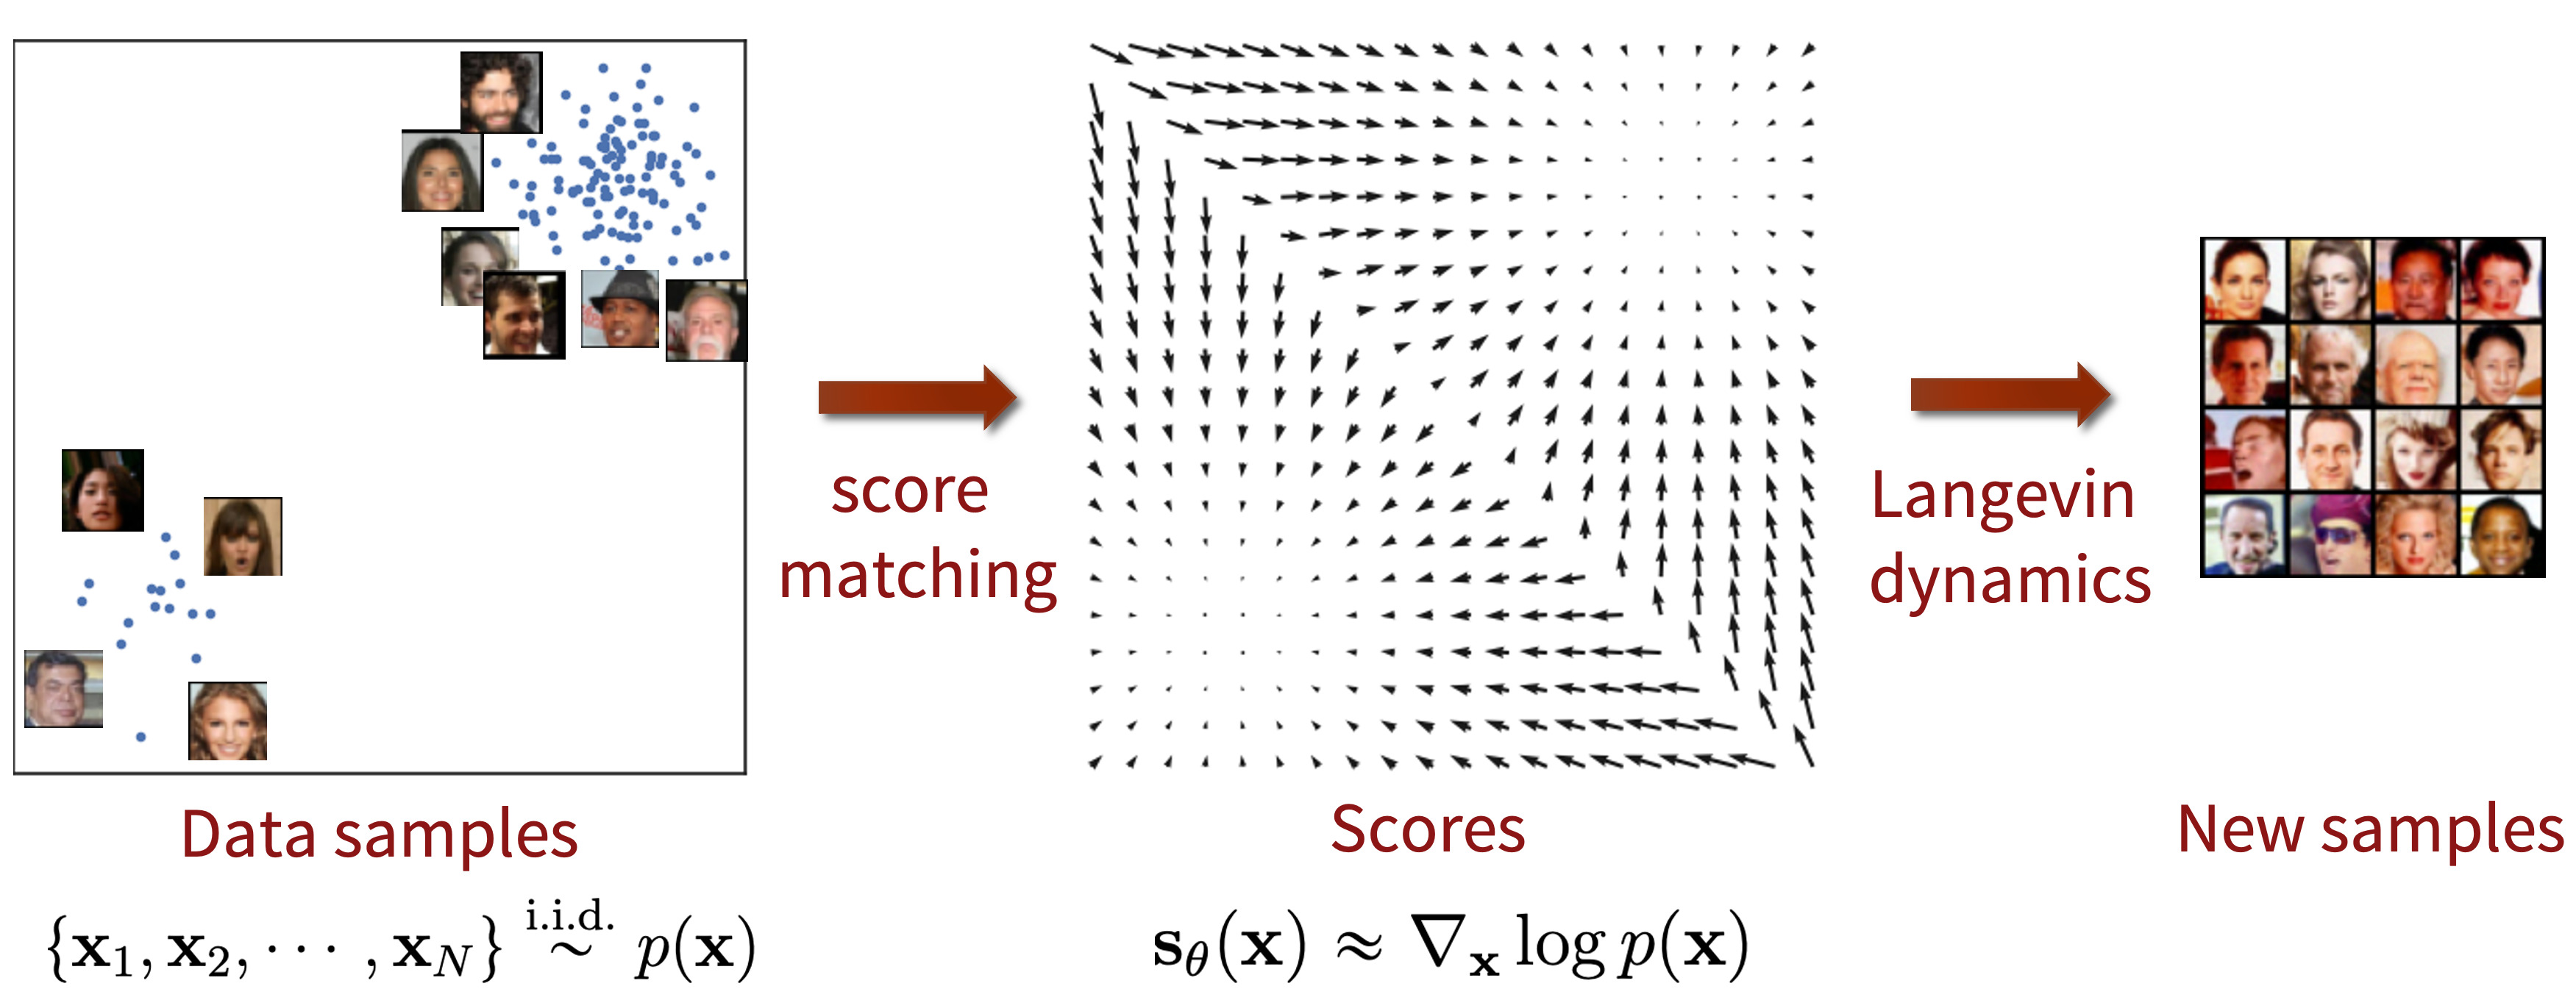
\includegraphics[width=\linewidth]{images/smld.jpg}

\end{frame}


% \begin{frame}{Score Matching}

% \begin{itemize}
%     \item Direction parametrise score $\mathbf{s}_\theta = \nabla_{\v{x}} \log p_\theta(x) = - U_\theta(x)$
%     \item Fisher divergence $\mathrm{D}_F(p_0~||~p_\theta) = \PE_{x \sim p_0}{\left[ \tfrac{1}{2} \| \nabla \log p_0(x) - \nabla \log p_\theta(x) \|^2  \right]}$
%     \item fitting score equivalent fitting density
%     \item Fisher divergence referred as \textbf{explicit score matching} loss \textit{impractical} as requires unknown $\nabla \log p_0(x)$
%     \item \textbf{Implicit score matching} \cite{hyvarinen2005}
%     $\mathrm{D}_F(p_0~||~p_\theta) = \PE_{x \sim p_0}{\left[ \tfrac{1}{2} \| \nabla \log p_\theta(x) \|^2 + \dive(\nabla \log p_\theta)(x) \right]} + \text{constant}$ 
%     \begin{itemize}
%         \item Slow mixing with Langevin algorithm (non-convex \cite{eberle2016reflection})
%         \item Poor score estimation
%     \end{itemize}
% \end{itemize}


% % \begin{itemize}
% % \item Weighted by $p(\v{x})$ -> poor fit weight $p$ is low
% % \item anneal / add gaussian noise -> but then fit wrong distribution
% % \item sequence of annealing
% % \end{itemize}

% \end{frame}

\begin{frame}{But this does not quite work...}
    \begin{center}
        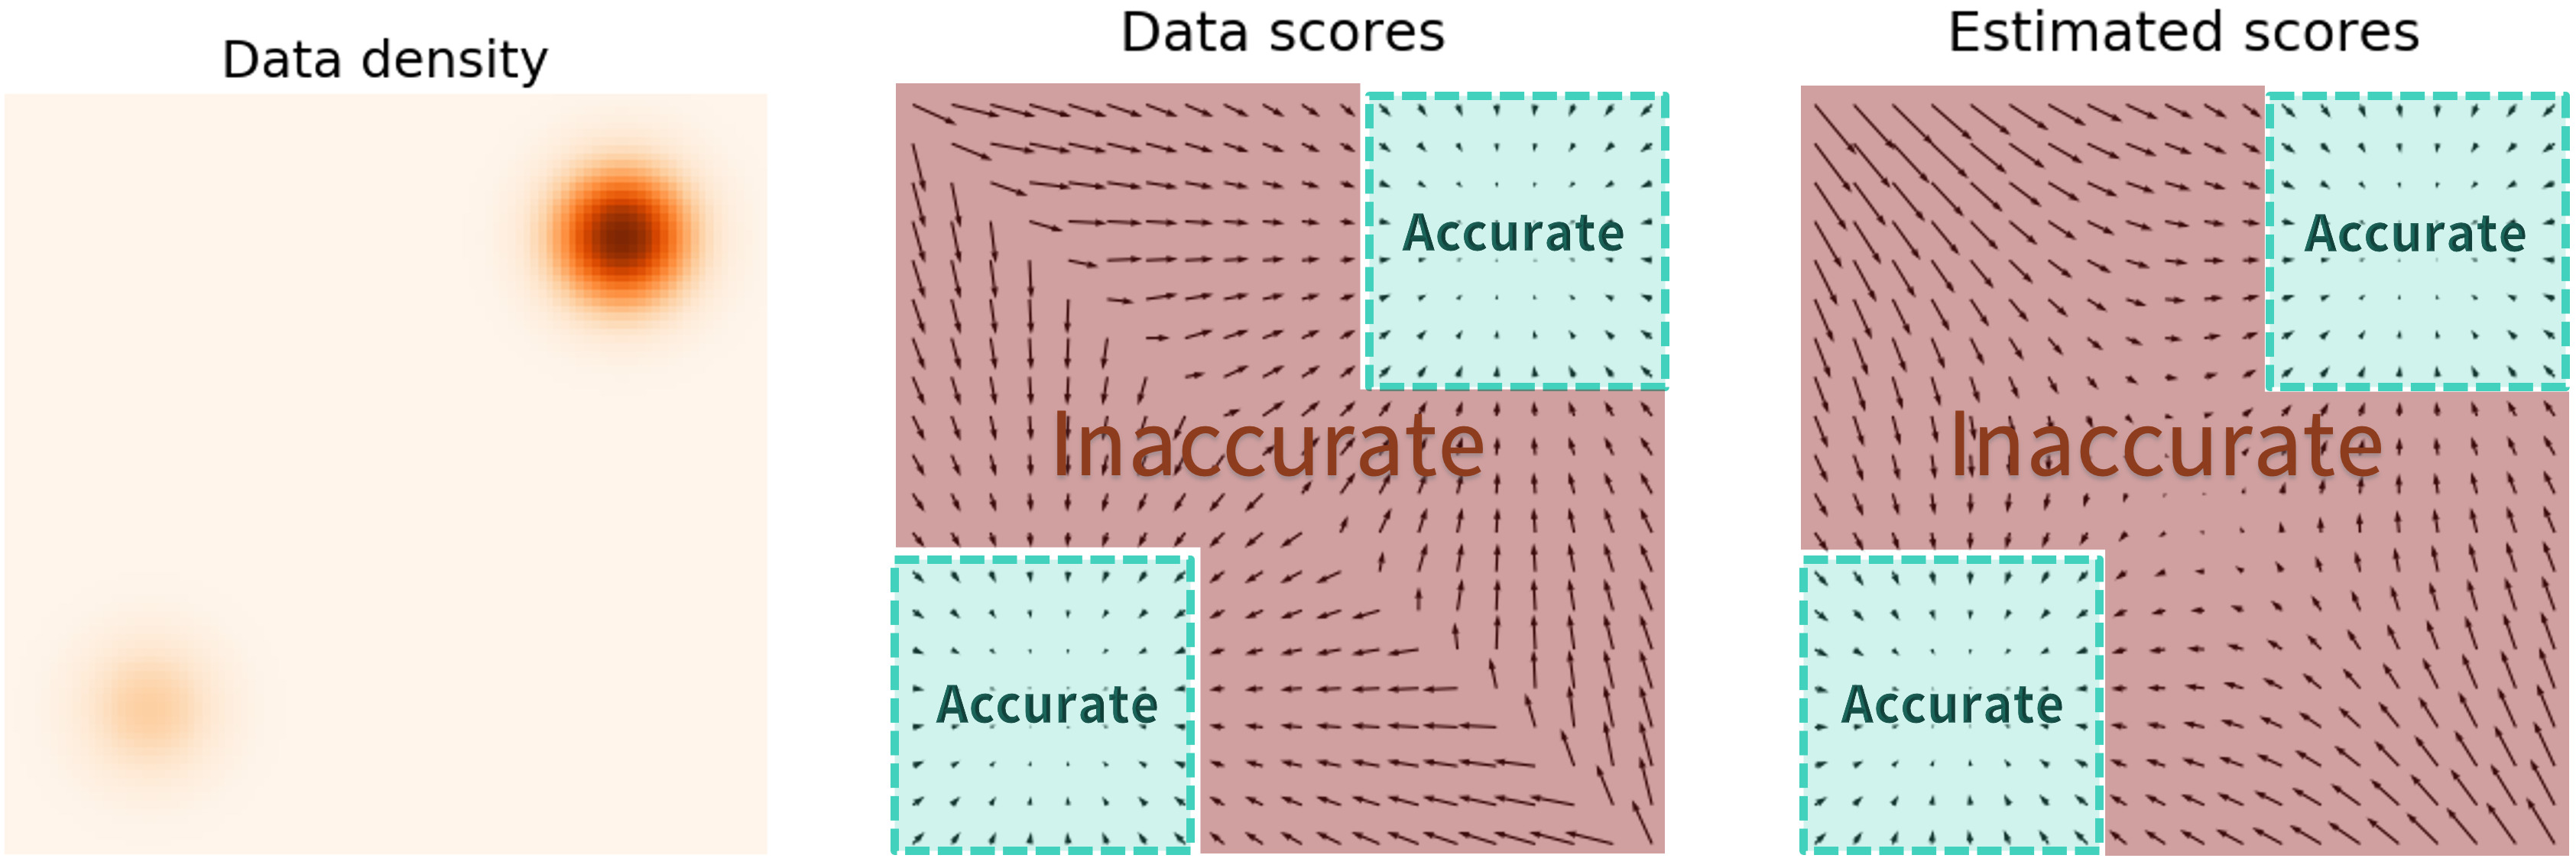
\includegraphics[width=0.8\linewidth]{images/pitfalls}
    \end{center}
    % Looking at the score matching objective, we see it will only learn the score at the datapoints.
    % \begin{equation}
    %     \ell_{\mathrm{esm}}(\hlyellow{\mathbf{s}_\theta}) = \E_{\hlred{\scriptstyle x \sim p(\v{x})}}\sbr{\norm{\nabla_{\v{x}} \log p(\v{x}) - \hlyellow{\mathbf{s}_\theta}(x)}^2},
    % \end{equation}
    % Because the data is supported on a finite set of samples this can fail if we can start with samples close to the data.
    \textbf{Issues}:
    \begin{itemize}
        % \item Score matching objectives are weighted by $\hlred{p(\v{x})}$ leading to \textit{poor score approximation} outside the support of $p$.
        \item \textit{Poor score approximation} outside the support of $p$.
        \item \textit{Slow mixing} with Langevin algorithm (non-convex \cite{eberle2016reflection}).
    \end{itemize}
\end{frame}


\section{Noising and denoising}

\begin{frame}{Denoising Score Matching \cite{vincent2011connection}}
% Lets put data density across the space by adding \textit{noise} to the data!
 \textbf{Solution}: Smoothing data density / spreading samples by adding \textit{noise} to the data!
\begin{equation*}
    % \hlblue{q(\tilde{x})} \triangleq \int q(\tilde{x} | x) p(\v{x}) dx, \quad \ell_{\mathrm{dsm}}(\hlyellow{\mathbf{s}_\theta}) \triangleq \E_{x \sim \hlblue{{\scriptstyle q(\tilde{x})}}}\sbr{\norm{\nabla_{\v{x}} \log p(\v{x}) - \hlyellow{\mathbf{s}_\theta}(x)}^2}
    \hlblue{p_\sigma(\tilde{\v{x}})} \triangleq \int p_\sigma(\tilde{\v{x}} | \v{x}) p(\v{x}) \rmd \v{x}, \ \
    \ell_{\mathrm{esm}}^{p_\sigma}(\hlyellow{\mathbf{s}_\theta})  \triangleq \E_{p_\sigma(\tilde{\v{x}})}\sbr{\norm{\nabla_{\tilde{\v{x}}} \log p_\sigma(\tilde{\v{x}}) - \hlyellow{\mathbf{s}_\theta}(\tilde{\v{x}})}^2}.
    % \ell_{\mathrm{dsm}}^{p_\sigma}(\hlyellow{\mathbf{s}_\theta}) \triangleq \E_{\v{x} \sim {{\scriptstyle p(\v{x}) p_\sigma(\tilde{\v{x}} | \v{x})}}}\sbr{\norm{\nabla_{\tilde{\v{x}}} \log p_\sigma(\tilde{\v{x}} | \v{x}) - \hlyellow{\mathbf{s}_\theta}(\tilde{\v{x}})}^2}.
\end{equation*}
\begin{center}
\includegraphics[width=0.8\linewidth]{images/single_noise.jpg}    
\end{center}
% Typically $p_\sigma(\tilde{\v{x}} | \v{x}) = \c{N}(\tilde{\v{x}}|\v{x}, \sigma^2) \Rightarrow \nabla_{\tilde{\v{x}}} \log p_\sigma(\tilde{\v{x}} | \v{x}) = \tfrac{{\v{x}} - \tilde{\v{x}}}{\sigma^2} = -\tfrac{\epsilon}{\sigma}$.
% Unfortunately we have to trade-off learning better scores and corrupting our data! 
% Yet, targeting wrong density $\hlblue{p_\sigma(\tilde{\v{x}})} \neq \hlred{p(\v{x})} \Rightarrow$ trade-off between small and large value of $\sigma$.

% \begin{itemize}
%     % \item Score matching losses are weighed by the data density $p_0$ which may be 0 or very low in some domain
%     % \item Learnt score will be poor on this domain resulting in poor samples from the Langevin dynamics
%     \item Idea: smooth data distribution with noise
%     \item Add some noise on data-points $\tilde{x} = x + \epsilon$ / annealing
%     \item $q(\tilde{x}) = \int q(\tilde{x}|x) p_0(x) \rmd x$, typically $q(\tilde{x}|x) = \mathrm{N}(\tilde{x}|x, \sigma^2)$.
%     \item $\mathrm{D}_F(p_0~||~p_\theta) = \PE_{\tilde{x},x \sim q}{\left[ \tfrac{1}{2} \| \nabla \log q(\tilde{x}|x) - \nabla \log p_\theta(x) \|^2  \right]} + \text{constant}$
%     \item Issue trade-off between overcoming noise vs learning wrong distribution
% \end{itemize}
% \todo[inline]{add figure from song's blog post}

\end{frame}

\begin{frame}{Proof of the denoising score matching loss}
The explicit score matching loss on the marginal distribution $\hlblue{p_\sigma(\tilde{\v{x}})}$ is given by
    \begin{align*}
        \ell_{\mathrm{esm}}^{p_\sigma}(\hlyellow{\mathbf{s}_\theta})  \triangleq \E_{p_\sigma(\tilde{\v{x}})}\sbr{\norm{\nabla_{\tilde{\v{x}}} \log p_\sigma(\tilde{\v{x}}) - \hlyellow{\mathbf{s}_\theta}(\tilde{\v{x}})}^2}
        = \E_{p_\sigma(\tilde{\v{x}})}\sbr{\norm{\hlyellow{\mathbf{s}_\theta}(\tilde{\v{x}})}^2} -  S(\theta) + C,
    \end{align*}
    \vspace{-0.8em}
    \begin{align*}
        \text{with}\ \ S(\theta) &= \E_{p_\sigma(\tilde{\v{x}})}\sbr{\innerprod{\hlyellow{\mathbf{s}_\theta}(\tilde{\v{x}})}{\nabla_{\tilde{\v{x}}} \log p_\sigma(\tilde{\v{x}})}}
        = \int_{\tilde{\v{x}}} p_\sigma(\tilde{\v{x}}) {\innerprod{\hlyellow{\mathbf{s}_\theta}(\tilde{\v{x}})}{\frac{\nabla_{\tilde{\v{x}}} p_\sigma(\tilde{\v{x}})}{p_\sigma(\tilde{\v{x}})}}} \rmd \tilde{\v{x}} \\
        &= \int_{\tilde{\v{x}}} {\innerprod{\hlyellow{\mathbf{s}_\theta}(\tilde{\v{x}})}{\nabla_{\tilde{\v{x}}} p_\sigma(\tilde{\v{x}})}} \rmd \tilde{\v{x}} \\
        &= \int_{\tilde{\v{x}}} {\innerprod{\hlyellow{\mathbf{s}_\theta}(\tilde{\v{x}})}{\nabla_{\tilde{\v{x}}} \int_{{\v{x}}} p_0(\v{x}) p_\sigma(\tilde{\v{x}}|\v{x}) \rmd \v{x}}} \rmd \tilde{\v{x}} \\
        &= \int_{\tilde{\v{x}}} {\innerprod{\hlyellow{\mathbf{s}_\theta}(\tilde{\v{x}})}{ \int_{{\v{x}}} p_0(\v{x}) p_\sigma(\tilde{\v{x}}|\v{x}) \nabla_{\tilde{\v{x}}} \log p_\sigma(\tilde{\v{x}}|\v{x}) \rmd \v{x}}} \rmd \tilde{\v{x}} \\
        % &= \int_{\tilde{\v{x}}} {\innerprod{\hlyellow{\mathbf{s}_\theta}(\tilde{\v{x}})}{ \int_{{\v{x}}} p_0(\v{x}) p_\sigma(\tilde{\v{x}}|\v{x}) \nabla_{\tilde{\v{x}}} \log p_\sigma(\tilde{\v{x}}|\v{x}) \rmd \v{x}}} \rmd \tilde{\v{x}} \\
        &= \E_{p_0(\v{x}) p_\sigma(\tilde{\v{x}}|\v{x})}\sbr{\innerprod{\hlyellow{\mathbf{s}_\theta}(\tilde{\v{x}})}{\nabla_{\tilde{\v{x}}} \log p_\sigma(\tilde{\v{x}}|\v{x})}}.
    \end{align*}
 $ \Rightarrow \ell_{\mathrm{esm}}^{p_\sigma}(\hlyellow{\mathbf{s}_\theta}) = \ell_{\mathrm{dsm}}^{p_\sigma}(\hlyellow{\mathbf{s}_\theta}) + C' 
= \E_{{{\scriptstyle p_0(\v{x}) p_\sigma(\tilde{\v{x}} | \v{x})}}}\sbr{\norm{\nabla_{\tilde{\v{x}}} \log p_\sigma(\tilde{\v{x}} | \v{x}) - \hlyellow{\mathbf{s}_\theta}(\tilde{\v{x}})}^2} + C'.$
\end{frame}

\begin{frame}{Denoising Score Matching \cite{vincent2011connection}}
    % Lets put data density across the space by adding \textit{noise} to the data!
     \textbf{Solution}: Smoothing data density / spreading samples by adding \textit{noise} to the data!
    \begin{equation*}
        % \hlblue{q(\tilde{x})} \triangleq \int q(\tilde{x} | x) p(\v{x}) dx, \quad \ell_{\mathrm{dsm}}(\hlyellow{\mathbf{s}_\theta}) \triangleq \E_{x \sim \hlblue{{\scriptstyle q(\tilde{x})}}}\sbr{\norm{\nabla_{\v{x}} \log p(\v{x}) - \hlyellow{\mathbf{s}_\theta}(x)}^2}
        \hlblue{p_\sigma(\tilde{\v{x}})} \triangleq \int p_\sigma(\tilde{\v{x}} | \v{x}) p(\v{x}) \rmd \v{x}, \ \
        % \ell_{\mathrm{esm}}^{p_\sigma}(\hlyellow{\mathbf{s}_\theta})  \triangleq \E_{p_\sigma(\tilde{\v{x}})}\sbr{\norm{\nabla_{\tilde{\v{x}}} \log p_\sigma(\tilde{\v{x}}) - \hlyellow{\mathbf{s}_\theta}(\tilde{\v{x}})}^2}.
        \ell_{\mathrm{dsm}}^{p_\sigma}(\hlyellow{\mathbf{s}_\theta}) \triangleq \E_{\v{x} \sim {{\scriptstyle p(\v{x}) p_\sigma(\tilde{\v{x}} | \v{x})}}}\sbr{\norm{\nabla_{\tilde{\v{x}}} \log p_\sigma(\tilde{\v{x}} | \v{x}) - \hlyellow{\mathbf{s}_\theta}(\tilde{\v{x}})}^2}.
    \end{equation*}
    \begin{center}
    \includegraphics[width=0.8\linewidth]{images/single_noise.jpg}    
    \end{center}
    Typically $p_\sigma(\tilde{\v{x}} | \v{x}) = \c{N}(\tilde{\v{x}}|\v{x}, \sigma^2) \Rightarrow \nabla_{\tilde{\v{x}}} \log p_\sigma(\tilde{\v{x}} | \v{x}) = \tfrac{{\v{x}} - \tilde{\v{x}}}{\sigma^2} = -\tfrac{\epsilon}{\sigma}$.
    % Unfortunately we have to trade-off learning better scores and corrupting our data! 
    Yet, targeting wrong density $\hlblue{p_\sigma(\tilde{\v{x}})} \neq \hlred{p(\v{x})} \Rightarrow$ trade-off between small and large value of $\sigma$.
    
    % \begin{itemize}
    %     % \item Score matching losses are weighed by the data density $p_0$ which may be 0 or very low in some domain
    %     % \item Learnt score will be poor on this domain resulting in poor samples from the Langevin dynamics
    %     \item Idea: smooth data distribution with noise
    %     \item Add some noise on data-points $\tilde{x} = x + \epsilon$ / annealing
    %     \item $q(\tilde{x}) = \int q(\tilde{x}|x) p_0(x) \rmd x$, typically $q(\tilde{x}|x) = \mathrm{N}(\tilde{x}|x, \sigma^2)$.
    %     \item $\mathrm{D}_F(p_0~||~p_\theta) = \PE_{\tilde{x},x \sim q}{\left[ \tfrac{1}{2} \| \nabla \log q(\tilde{x}|x) - \nabla \log p_\theta(x) \|^2  \right]} + \text{constant}$
    %     \item Issue trade-off between overcoming noise vs learning wrong distribution
    % \end{itemize}
    % \todo[inline]{add figure from song's blog post}
    
    \end{frame}
    

\begin{frame}{Multiple noise  perturbations \cite{song2019generative,song2020improved}}

% We can alleviate this by having \textit{multiple} scales. A series of scales guides us towards the data.
% Solution: \textbf{annealed Langevin} dynamics with \textit{multiple} scales $\sigma_1 < \dots < \sigma_M$.
% Solution: Using \textit{multiple increasing} noise scales $0 \approx \sigma_1 < \dots < \sigma_T \gg 1$: 
Solution: Using \textit{multiple} scales $ \sigma_0 < \dots < \sigma_T$: 
$\hlblue{p_{\sigma_t}(\tilde{\v{x}})} \triangleq \int p_{\sigma_t}(\tilde{\v{x}} | \v{x}; \sigma_t) p(\v{x}) \rmd \v{x}$.
\begin{figure}
    \centering
    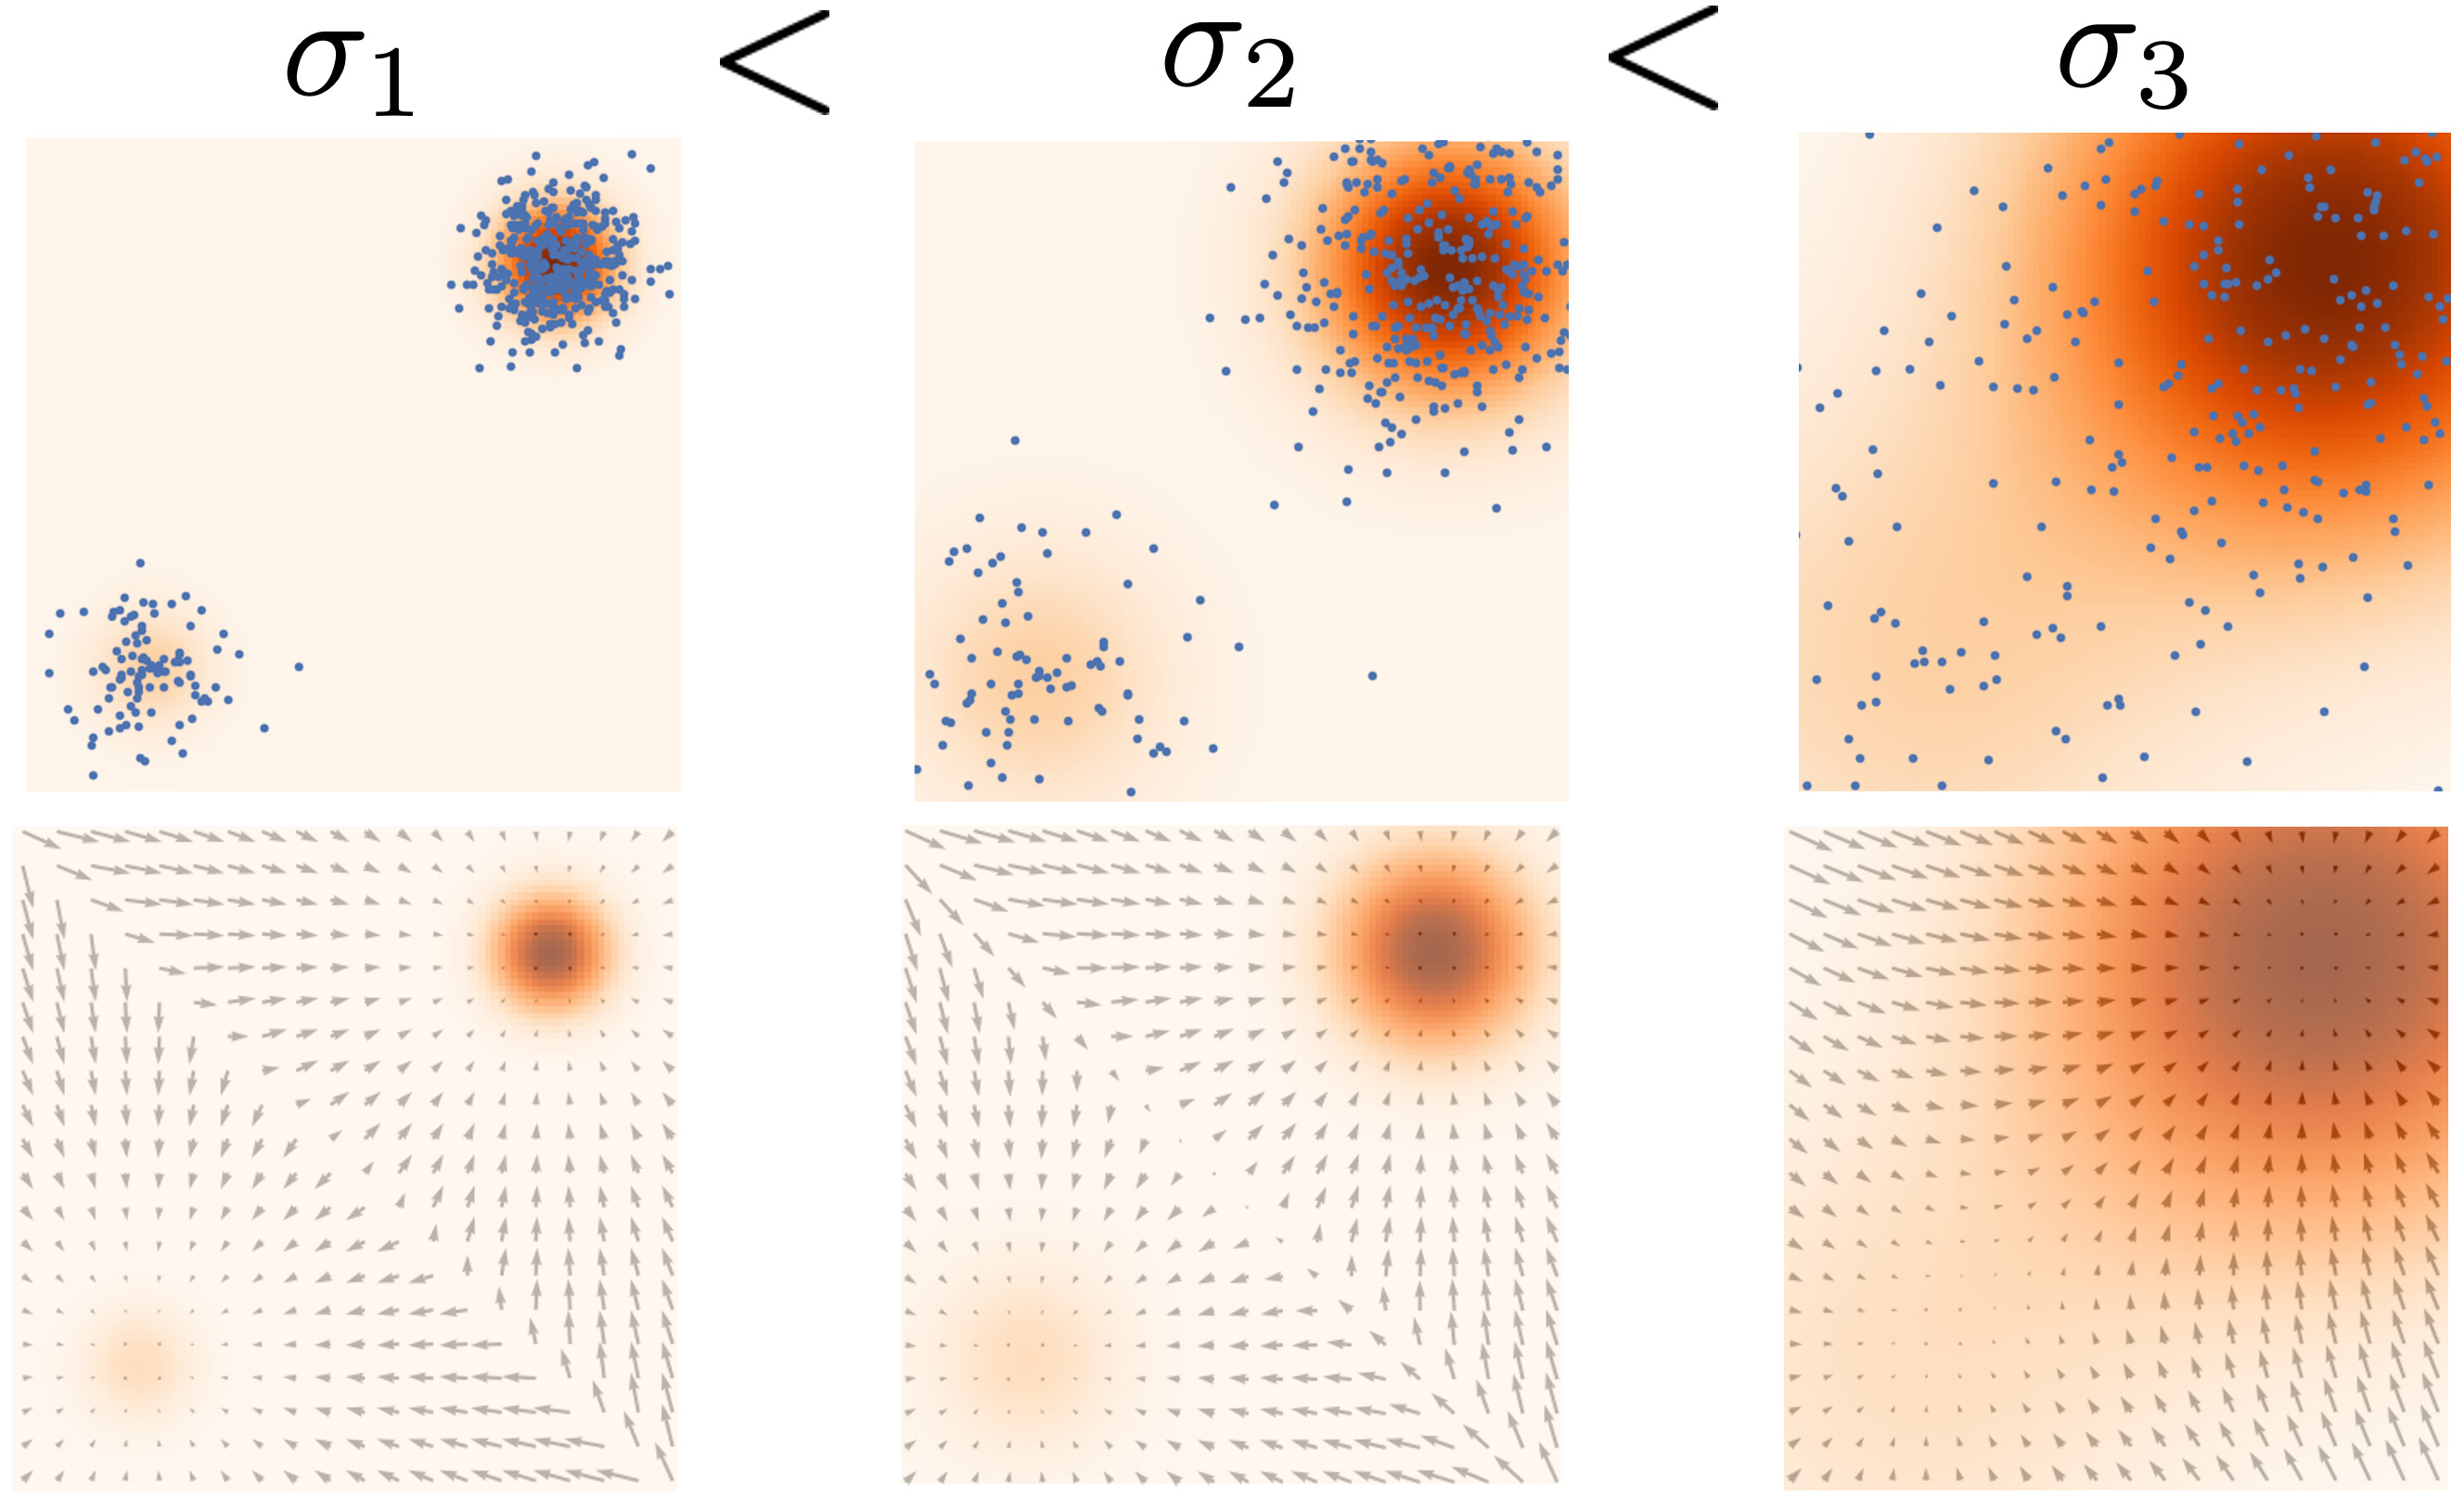
\includegraphics[height=0.5\textheight]{images/multi_scale.jpg}
\end{figure}
\vspace{-0.5em}
Score matching with Langevin dynamics (SMLD):
Parameterise a score network $\hlyellow{s_\theta}(\sigma_t, \v{x})$ indexed by the noise scale $\sigma_t$:
\vspace{-0.5em}
\begin{equation*}
    \ell_{\mathrm{smld}}(\hlyellow{\mathbf{s_\theta}}) 
    \triangleq \sum_{t=0}^T \lambda(t) \ell_{\mathrm{dsm}}^{p_{\sigma_t}}(\hlyellow{\mathbf{s}_\theta}) 
    = \sum_{t=0}^T \lambda(t) \E_{\v{x} \sim p_{\sigma_t}(\v{x})} \sbr{\norm{\nabla_{\tilde{\v{x}}} \log p_{\sigma_t}(\tilde{\v{x}} | \v{x}) - \hlyellow{\mathbf{s_\theta}}(\sigma_t, \v{x})}^2}.
\end{equation*}
% \begin{itemize}
%     \item overcoming the noise trade-off with \textbf{annealed} Langevin dynamics
%     \item $q_{\sigma_i}(\tilde{x}) = \int \mathrm{N}(\tilde{x}|x, \sigma_i^2) p_0(x) \rmd x$.
%     \item Increasing sequence of noise $\sigma_0<\dots<\sigma_L$
%     \item Noise Conditional Score-Based Model (NCSM) $\mathbf{s}_\theta(i, x) \approx \nabla \log q_{\sigma_i}({x})$
%     \item loss $\sum_{i=1}^L \lambda\PE_{\tilde{x},x \sim q}{\left[ \tfrac{1}{2} \| \nabla \log q(\tilde{x}|x) - \nabla \log p_\theta(x) \|^2  \right]}$
%     \item add algorithm?
% \end{itemize}
% \todo[inline]{add figure from song's blog post}
\end{frame}

\begin{frame}{Sampling from multiple noise scales}
    Sample with \textbf{annealed Langevin} dynamics:
    \begin{enumerate}
        \item Start with large $\sigma_T$ and target $p_{\sigma_T}$ with Langevin dynamics.
        \item Decrease noise $\sigma_{T-1} < \sigma_T$ and \textit{warm-start} with previous samples:
        % \begin{equation}
            % $\quad \bfX^{k+1}_t = \bfX_t^k + \gamma_t \hlyellow{\mathbf{s_\theta}}\del{\sigma_t, \bfX^k_t} + \sqrt{2\gamma_t} \bfZ^{k+1}_t$
            % and $\bfX^{0}_{t-1} = \bfX^{K}_t$.
        % \end{equation}
        \item Repeat procedure until $\sigma_0$ is very small so that $p_{\sigma_0} \approx p$.
    \end{enumerate}
    
    \begin{center}
        \animategraphics[autoplay,loop,width=0.8\textwidth]{10}{images/ald/ald-}{0}{152}
    \end{center}
    
    % We start with samples from some prior distribution, and use the samples from each noise scale as the initialisation for the next.
    % This not dissimilar idea to SMC methods. CRAFT \cite{matthews2022continual} is perhaps a similar line of thought in that direction.
\end{frame}


% \begin{frame}{Relation with time-reversal}
\begin{frame}{Annealing Langevin dynamics}
%
%   \small
\vspace{-.2em}
  \begin{algorithm}[H]
  \begin{algorithmic}[1]
  \small
    \State \textbf{Input:} $\{\sigma_t\}_{t=1}^T$, $\{\gamma_t\}_{t=1}^T$, $K$
    \State Initialize $\bfX_{T}^0 \sim \mathcal{N}(0, \sigma_T \Id)$.
    \For{$t=T$ to $1$}
    \For{$k=0$ to $K-1$}
    \State Sample $\bfX_{t}^{k+1} = \bfX_{t}^k + \gamma_t \hlyellow{\mathbf{s}_\theta}(\sigma_t, \bfX_t^k) + \sqrt{2 \gamma_t} Z_t^{k+1}$
    \EndFor
    \State $X_{t-1}^0 = X_{t}^K$
    \EndFor
    % \State \textbf{Return} $\bfX_0^0$.
\end{algorithmic}
\caption{\small Sampling of annealing Langevin dynamics}
\label{alg:seq}
\end{algorithm}
% \vspace{-1.5em}
\vspace{-1.2em}
% \small
% Set $K=1$, $\gamma_t = \gamma$ and $\sigma_t^2 = t \gamma$.
% \vspace{-.5em}
% \begin{itemize}
%     \item \textbf{Noising}
%     \begin{itemize}
%     \item Update: $\bfX_{t+1} = \bfX_t + \sqrt{2 \gamma} \bfZ_{t+1}$ with $\bfZ_{t+1} \sim \mathcal{N}(0,\Id)$.
%     \item Kernel: $p_{t+1|t}(x_{t+1}|x_{t}) = \mathcal{N}(x_{t}, {2 \gamma})$.
%     \end{itemize}
%     \item \textbf{Denoising}
%     \begin{itemize}
%     \item Udapte: $\bfX_{t} = \bfX_{t+1} + \gamma \hlyellow{\mathbf{s}_\theta}(\sigma_{t+1}, \bfX_{t+1}) + \sqrt{2 \gamma} \bfZ_{t+1}$.
%     \item Kernel: $p_{t|t+1}(x_{t}|x_{t+1}) = \mathcal{N}(x_{t+1} + \gamma \hlyellow{\mathbf{s}_\theta}(\sigma_{t+1}, x_{t+1}), {2 \gamma})$.
%     \end{itemize}
% \end{itemize}
   
\end{frame}


\begin{frame}{This really works!}
    \begin{center}
        \animategraphics[autoplay,loop,width=0.4\textwidth]{10}{images/celeba_large/celeba_large-}{0}{49}
        \hspace{2em}
        \animategraphics[autoplay,loop,width=0.4\textwidth]{10}{images/cifar10_large/cifar10_large-}{0}{49}
    \end{center}
\end{frame}

\begin{frame}{Recap: SMLD}
 %
 \begin{center}
        \includegraphics[width=\textwidth]{images/ald/ald-152.png}
    \end{center}
\begin{itemize} \setbeamertemplate{itemize items}[triangle]
    \item Choose increasing sequence of \textbf{noise} $\sigma_t$.
    \item Construct noised distribution $p_{\sigma_t}$.
    \item Fit amortised score network $\hlyellow{\mathbf{s}_\theta}(\sigma_t, x_t)$ to approximate true score $\nabla \log p_{\sigma_t}(x_t)$.
    \item Sample with \textbf{annealed Langevin} dynamics.
\end{itemize}
%
\end{frame}
